\section{Aufgabe 4 - Entprell-Automat}
\subsection{Entwurf}
	\paragraph{State-Machine-Charts}\hfill \\

	\paragraph{LED} enthält die Komponente Entprellung und verbindet die Ein- und Ausgangssignale. (\ref{lst:04-led}~LED.vhdl-Code) \\
	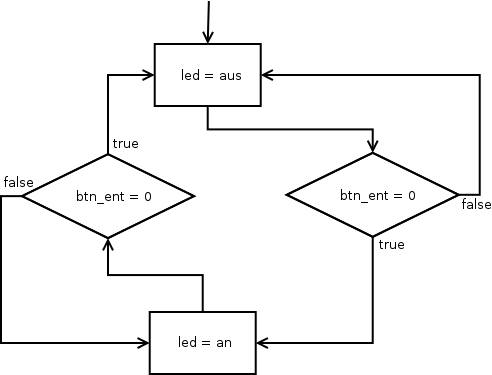
\includegraphics[width=0.7\textwidth]{\Path/resources/04-led.png}
	
	\paragraph{Entprellung} enthält die Komponente Zaehler, der bei der Veränderung des Eingangsignals gestartet wird und für 3ms weitere Änderungen ignoriert. (\ref{lst:04-entprellung}~Entprellung.vhdl-Code) \\
	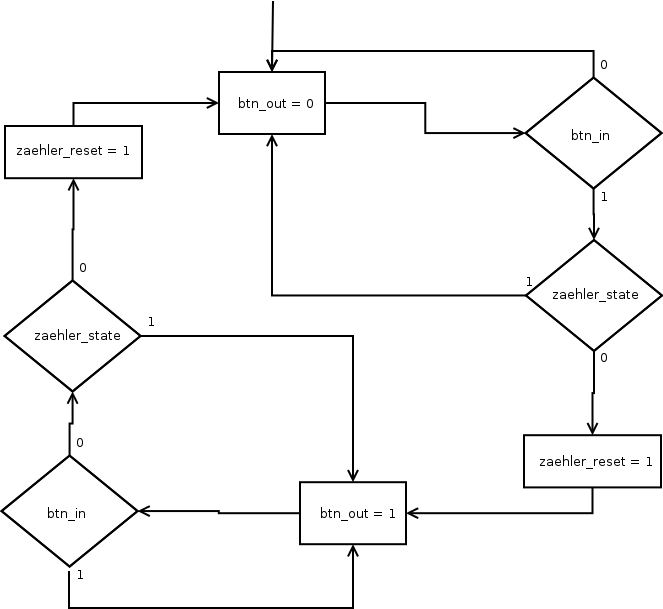
\includegraphics[width=0.8\textwidth]{\Path/resources/04-entpreller.png}


	\paragraph{Zaehler} implementiert einen Zähler, der durch ein Signal definierte Schritte zählt. Ausgegeben wird der aktuelle Zustand des Zählers. Eingegeben ein Reset-Signal. (\ref{lst:04-zaehler}~Zaehler.vhdl-Code) 
	\paragraph{Kopplung} \hfill\\
	Es wird eine synchrone Automatenkopplung über die Ausgangssignale mit einem Taktsignal verwendet.


\subsection{Auswertung}
	\paragraph{Ressourcenbedarf}
	\begin{itemize} 
	\item 86 Logik-Elemente
	\item davon 79 dedizierte Logik-Elemente
	\item 44 Register
	\item 3 Pins 
	\item maximale Taktfrequenz von 178 MHz
	\end{itemize}
